% !TEX root = ../main.tex
\chapter{结果对比}
本章主要进行了绘制效果,算法效率,算法精度这三方面的对比,我们进行对比实验的硬件条件如下:CPU为英特尔酷睿i7 4710MQ@2.50GHz,GPU为英伟达GeForce GT 730M,内存大小为8GB。对比的对象是传统的自由变形\cite{Sederberg86}和光滑自由变形\cite{Cui15}。选用的变形空间均为B样条体,其次数为$3\times3\times3$,控制顶点个数为$6\times6\times6$。为了方便比较,待变形的模型顶点都将先归一化到$[-1, 1]^3$

由于光滑自由变形和本文算法最终的变形结果均为三角Bézier曲面片,本文采取与光滑自由变形相同的方案可视化这些曲面片,即均匀细分成三角形然后通过OpenGL绘制。用户可以通过参数控制三角Bézier曲面片的细分粒度,以将解析结果细分成不同精度的三角网格模型。在本章的实验中,所有三角Bézier曲面片都将被均匀细分成100个小三角形进行绘制。同时在比较光滑自由变形和本文方法的拟合误差时,误差值也将通过比较细分后三角形顶点的属性得到的。

在以下对比实验中,本文方法在分割阶段时,$l$的值固定为$\frac{1}{3}$的节点盒长度。

\section{绘制效果比对}
本节主要对比传统自由变形、光滑自由变形以及本文算法的绘制效果。对比实验的硬件环境与算法参数如上文所述。实验中选用帆船作为对比模型,该模型中包含了各种大小、各种形状的三角形,能够有效的检验变形算法产生结果的质量。

\autoref{subfig:renderer_effect}中展示了各个方法的绘制结果,\autoref{subfig:renderer_effect1}是传统自由变形的结果,可以很明显的看到帆船桅杆部分因采样密度不足造成的走样问题。光滑自由变形(\autoref{subfig:renderer_effect3})和本文方法(\autoref{subfig:renderer_effect2})均很好的解决了这一问题。

同时通过比较\autoref{subfig:renderer_effect3}和\autoref{subfig:renderer_effect2},可以发现本文算法和光滑自由变形的结果,从视觉上基本无法区分。\autoref{subfig:renderer_effect4}是本文方法和光滑自由变形的像素层面上的差异。红色的深度越深表示差异越大。白色表示没有差异。\autoref{subfig:renderer_effect3}和\autoref{subfig:renderer_effect2}的像素用256阶灰度表示,除去背景像素,两者像素值平均差异是$0.249$,最大差异是$51$。其中灰度差异小于5的像素点了占了总像素点的$99.02\%$。所以肉眼几乎无法看出两者差别。

通过以上分析,可以认为本文方法达到了和光滑自由变形相同的绘制效果。
\begin{figure}[htbp]
	\centering
	\begin{subfigure}[b]{.4\textwidth}
		\centering
		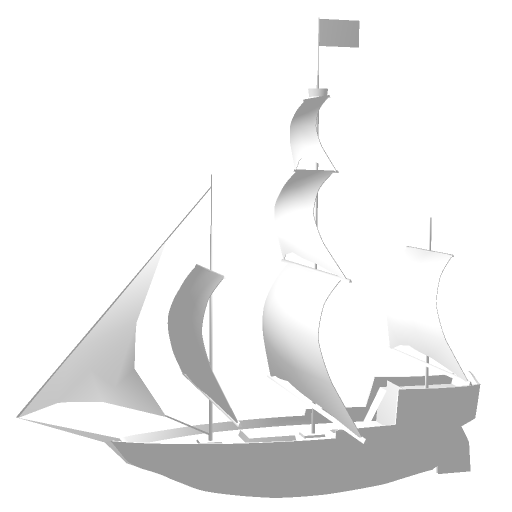
\includegraphics[width = \textwidth]{renderer_effect0.png}
		\caption{原始模型}\label{subfig:renderer_effect0}
	\end{subfigure}
	\quad
	\begin{subfigure}[b]{.4\textwidth}
		\centering
		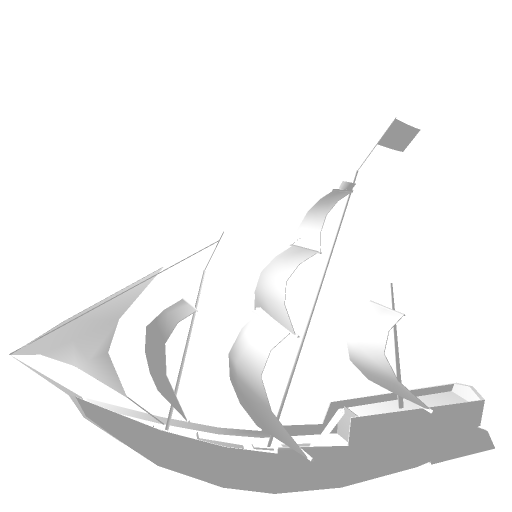
\includegraphics[width = \textwidth]{renderer_effect1.png}
		\caption{传统自由变形结果}\label{subfig:renderer_effect1}
	\end{subfigure}

	\centering
	\begin{subfigure}[b]{.4\textwidth}
		\centering
		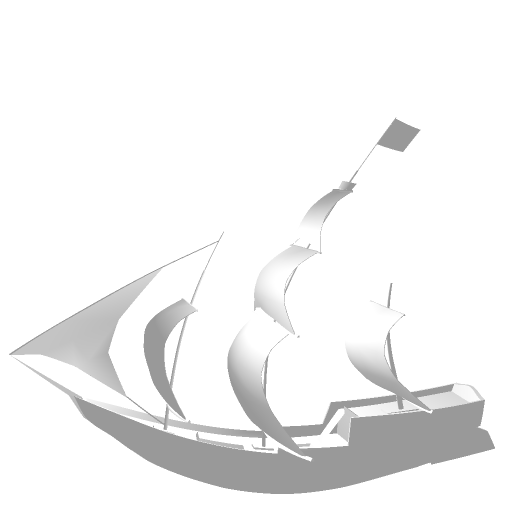
\includegraphics[width = \textwidth]{renderer_effect3.png}
		\caption{光滑变形结果}\label{subfig:renderer_effect3}
	\end{subfigure}
	\quad
	\begin{subfigure}[b]{.4\textwidth}
		\centering
		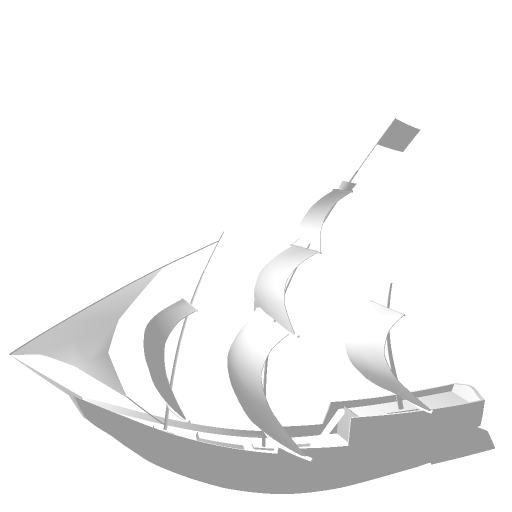
\includegraphics[width = \textwidth]{renderer_effect2.png}
		\caption{本文方法结果}\label{subfig:renderer_effect2}
	\end{subfigure}

	\centering
	\begin{subfigure}[b]{.4\textwidth}
		\centering
		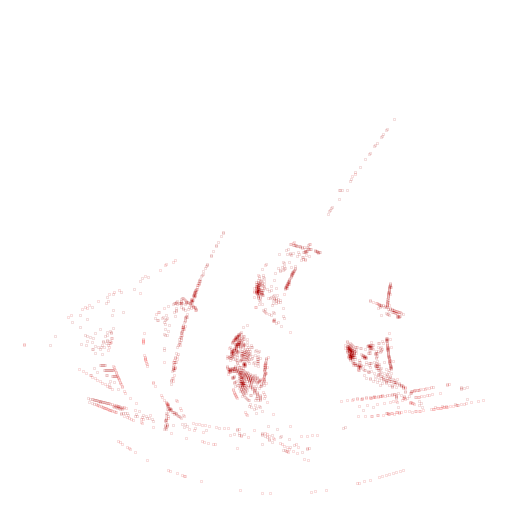
\includegraphics[width = \textwidth]{renderer_effect4.png}
        \caption{\autoref{subfig:renderer_effect3}和\autoref{subfig:renderer_effect2}的像素差异}\label{subfig:renderer_effect4}
	\end{subfigure}
	\quad
	\begin{subfigure}[b]{.4\textwidth}
		\centering
		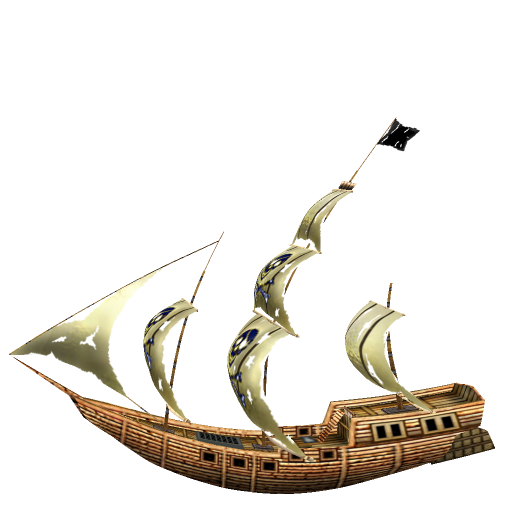
\includegraphics[width = \textwidth]{renderer_effect5.png}
		\caption{带纹理的本文结果}\label{subfig:renderer_effect5}
	\end{subfigure}
	\caption{绘制效果对比图}\label{subfig:renderer_effect}
\end{figure}

\section{效率对比}
本节的比较的对象仍然是光滑自由变形,选用的模型是一个高精度的蜗牛模型,如\autoref{fig:speed_compare}所示,由46742个面片组成。

\begin{figure}[htbp]
	\centering
	\begin{subfigure}[b]{.4\textwidth}
		\centering
		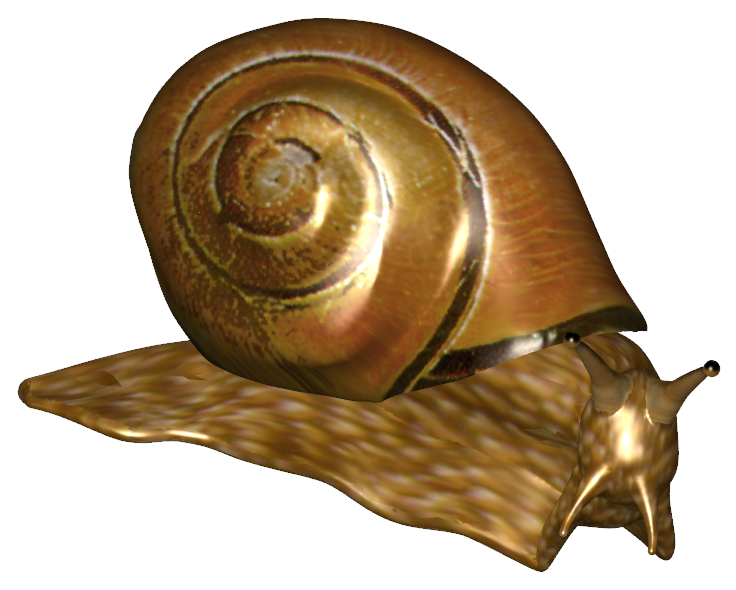
\includegraphics[width = \textwidth]{snail1.png}
		\caption{光滑自由变形绘制结果}\label{subfig:snail1}
	\end{subfigure}
	\quad
	\begin{subfigure}[b]{.4\textwidth}
		\centering
		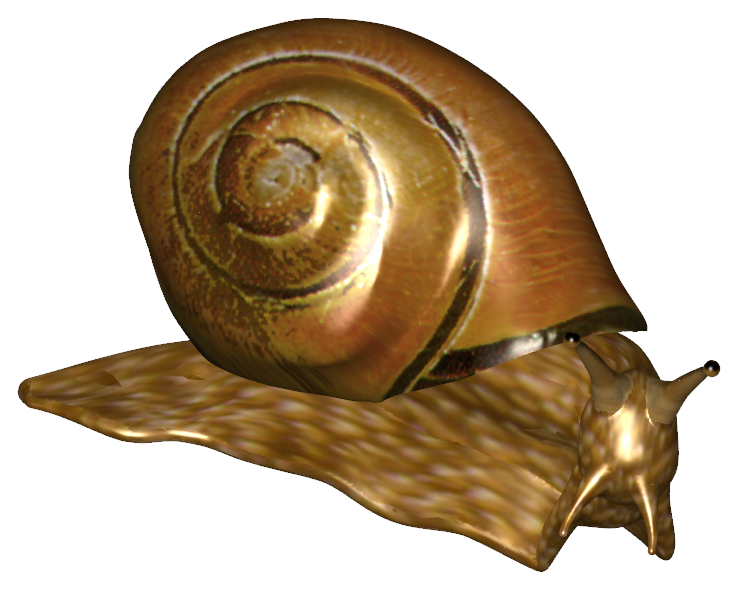
\includegraphics[width = \textwidth]{snail2.png}
		\caption{本文方法绘制结果}\label{subfig:snail2}
	\end{subfigure}
	\caption{效率对比采用的蜗牛模型}\label{fig:speed_compare}
\end{figure}

\subsection{分割阶段}
光滑自由变形的分割阶段在CPU中完成,本文方法在GPU中完成。\autoref{tab:clip_time_compare}中是两种方法在分割阶段所用的时间,本文方法具有较大优势,速度上快了近200倍。这其中在两方面的原因,一方面我们通过以空间换时间的策略,对较为耗时的“计算分割方案”这一过程进行了预计算。另一方面是我们用GPU实现了分割过程,而光滑自由变形是在CPU中实现的。

\begin{table}[htbp]
    \centering
    \caption{三角形分割阶段运行时间对比(单位:ms)}\label{tab:clip_time_compare}
    \begin{tabular}{lrr}
    \toprule
    \textbf{步骤}   & \textbf{本文方法} & \textbf{光滑自由变形\cite{Cui15}} \\
    \midrule
    生成PN三角形    & 4.618             & 104.465                           \\
    切割原始三角面片& 21.475            & 5027.418                          \\
    \midrule
    \textbf{总计}   & 26.093            & 5131.883                          \\
    \bottomrule
    \end{tabular}
\end{table}

\subsection{变形、绘制阶段}
变形过程又分为几个以下几个子过程:
\begin{enumerate}
    \item 计算拟合点。
    \item 计算约束点。
    \item 计算三角Bézier曲面片的控制顶点。
    \item 调整控制顶点。
\end{enumerate}

绘制也可以分为两个子过程:
\begin{enumerate}
    \item 离散化三角Bézier曲面片。
    \item 绘制。
\end{enumerate}

其中,绘制交由OpenGL流水管线实现,故不比较这一过程的时间。其它过程计算时间如\autoref{tab:deformation_time_compare}所示。

\begin{table}[htbp]
    \centering
    \caption{三角形变形、绘制阶段运行时间对比(单位:ms)}\label{tab:deformation_time_compare}
    \begin{tabular}{lrr}
    \toprule
    \textbf{步骤}     & \textbf{本文方法} & \textbf{光滑自由变形\cite{Cui15}} \\
    \midrule
    计算采样点位置     & \multirow{6}{*}{67.419} & 41.369     \\
    计算三角Bézier曲面片控制顶点      &                         & 11.125     \\
    计算三角Bézier曲面片的法向量场   &                         & 4.209     \\
    微调控制顶点         &                         & 4.344     \\
    离散三角Bézier曲面片 &                         & 4.057     \\
    \midrule
    \textbf{总计}& 67.419  & 65.464    \\
    \bottomrule
    \end{tabular}
\end{table}
本文采用OpenGL Compute Shader实现,为了尽可能提高运行效率,\autoref{tab:deformation_time_compare}中的几个阶段实现在了同一个Shader中,所以以上几个阶段本文方法只给出了总运行时间。

光滑自由变形由CUDA实现,该方法在实现上述过程时,大量的采用了大矩阵乘法,并交由cuBLAS计算。cuBLAS是CUDA官方提供的线性运算库,在相同的硬件下,实现相同的计数任务,用户自己编写的程序很难在时间效率上超过cuBLAS。所以我们有理由将光滑自由变形的变形过程所用的时间作为一个性能的标杆。本文以之为目标,作了很多算法及语言层面上的优化。最终得到的结果只比光滑自由变形慢了$2.99\%$。考虑到我们的算法采用的OpenGL Compute Shader实现,OpenGL Compute Shader并末提供大矩阵运算库,无法从大矩阵运算中得益,所以我们认为本文变形所用的时间是一个较为合理的结果。

\subsection{总结}
综上所述,在变形、绘制阶段,本文算法基本能达到和光滑自由变形相同的运行速度。而在分割阶段,本文方法具有较大优势,约比光滑自由变形快了近200倍。

\section{精度对比}
虽然光滑自由变形基于精确自由变形,但是该方法最终变形结果是通过用低次的三角Bézier曲面片拟合高次的精确结果得到,这样虽然提高了算法的运行效率,但同时也引入了法向和几何上的误差。本文方法也存在相同的拟合误差,并且本文未沿节点盒切割原始三角面片,这也是一个误差增加的潜在因素。本节希望通过误差分析说明本文方法的误差相较于自由变形并不会有显著增加。

本节中,本文方法的比较对象仍是光滑自由变形,我们分别计算光滑自由变形、本文方法的变形结果与精确结果的差异以得到两种方法对应的误差值。与光滑自由变形一样,本文方法也会通过法向信息微调三角Bézier曲面片的控制顶点。所以我们需要几何与法向都精确的模型作为本节实验变形所用的模型。为此我们选择了一个标准的立方体和一个由36个三次Bézier曲面组成的Utah茶壶作为变形模型进行误差分析,如\autoref{fig:error_ori}所示。标准立方体的精确变形结果可以通过精确自由变形\cite{Feng00}得到,Utah茶壶的精确变形结果可以通过传统FFD结合均匀加密采样得到。由于Utah茶壶是由Bézier曲面片组成的,所以必须先转化成多边形网格才能作为变形算法的输入,我们采用Casteljau细分算法\cite{farin2000essentials}将其转化成多边形网格。

\begin{figure}[htbp]
	\centering
	\begin{subfigure}[b]{.4\textwidth}
		\centering
		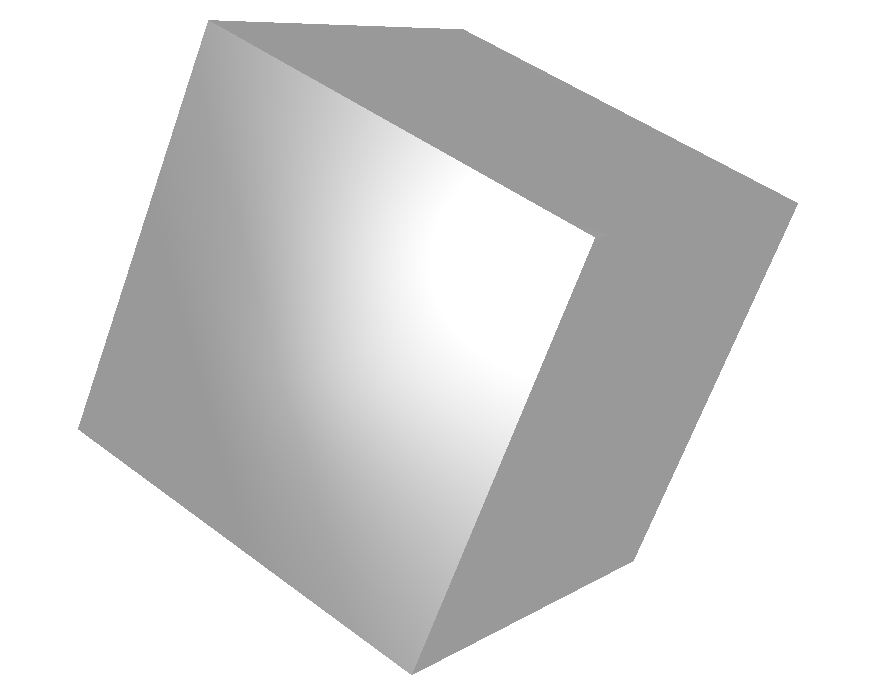
\includegraphics[width = \textwidth]{cube0.png}
		\caption{立方体}\label{subfig:cube0}
	\end{subfigure}
	\quad
	\begin{subfigure}[b]{.4\textwidth}
		\centering
		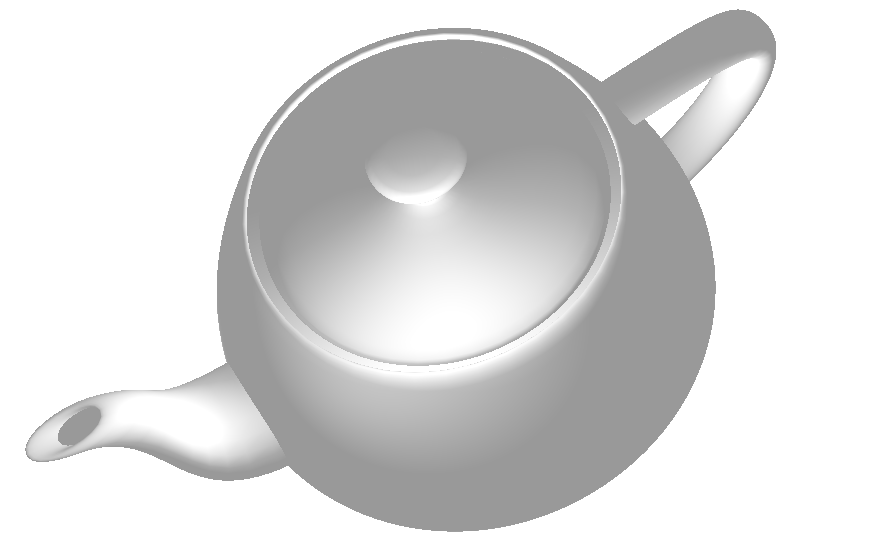
\includegraphics[width = \textwidth]{teapot0.png}
		\caption{Utah茶壶}\label{subfig:teapot0}
	\end{subfigure}
	\quad
	\caption{误差估计采用的模型}\label{fig:error_ori}
\end{figure}

\autoref{fig:cube_result}和\autoref{fig:teapot_result}是分别是立方体和Utah茶壶的在各个变形方法下的变形结果。

\begin{figure}[htbp]
	\centering
	\begin{subfigure}[b]{.3\textwidth}
		\centering
		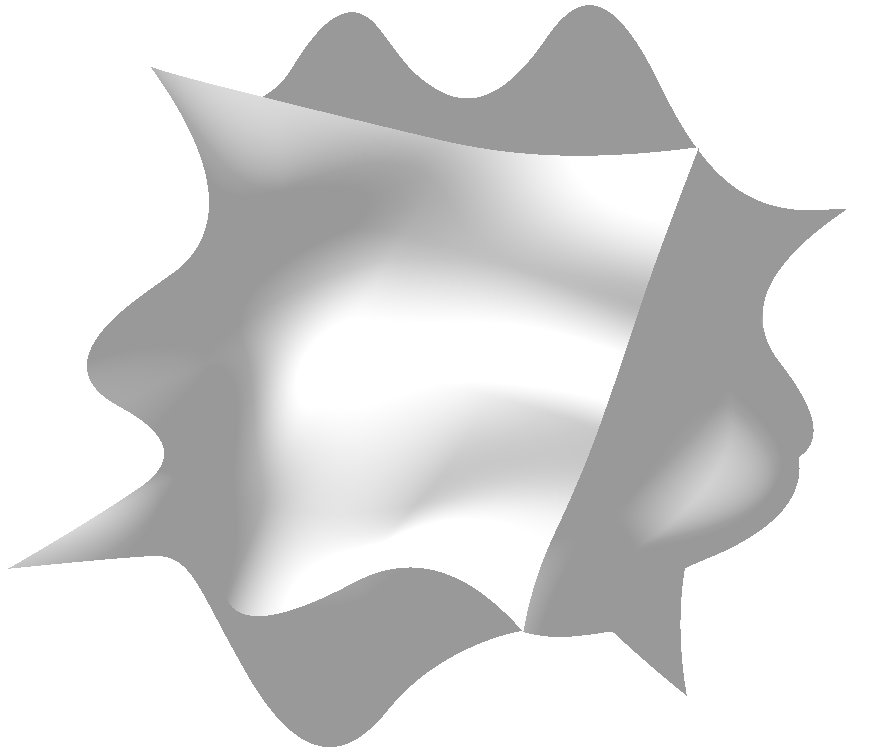
\includegraphics[width = \textwidth]{cube1.png}
		\caption{精确自由变形结果}\label{subfig:cube1}
	\end{subfigure}
	\begin{subfigure}[b]{.3\textwidth}
		\centering
		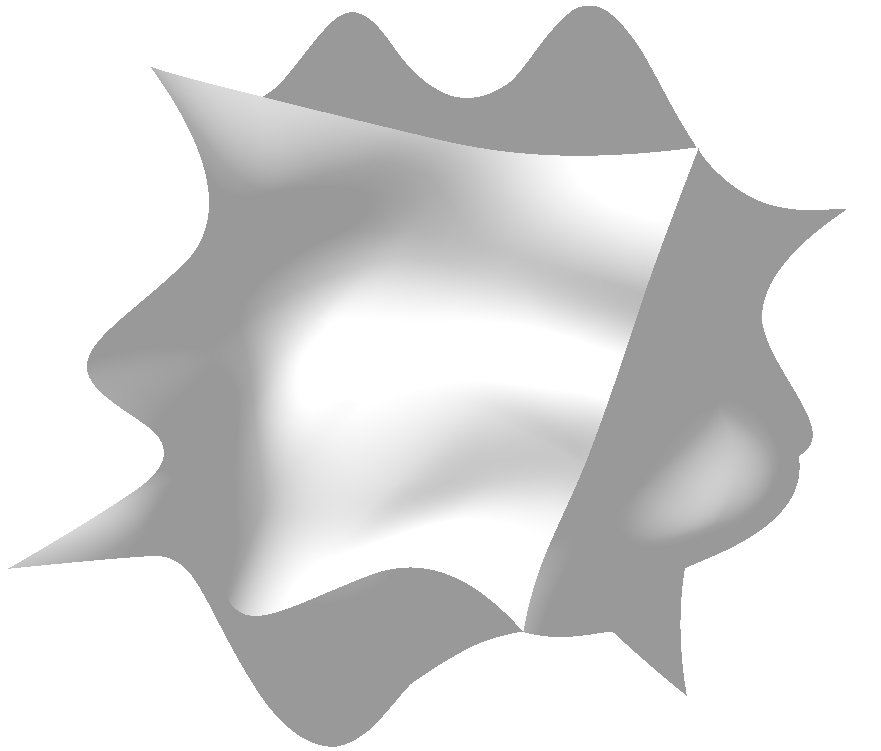
\includegraphics[width = \textwidth]{cube2.png}
		\caption{光滑自由变形结果}\label{subfig:cube2}
	\end{subfigure}
	\begin{subfigure}[b]{.3\textwidth}
		\centering
		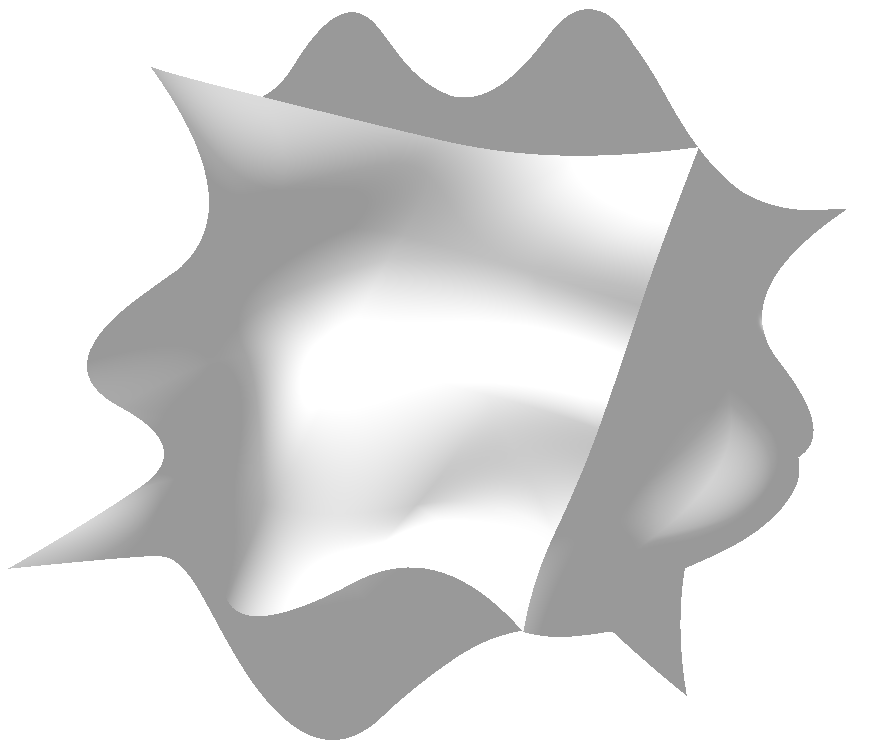
\includegraphics[width = \textwidth]{cube3.png}
		\caption{本文结果}\label{subfig:cube3}
	\end{subfigure}
	\caption{立方体变形结果}\label{fig:cube_result}
\end{figure}

\begin{figure}[htbp]
	\centering
	\begin{subfigure}[b]{.3\textwidth}
		\centering
		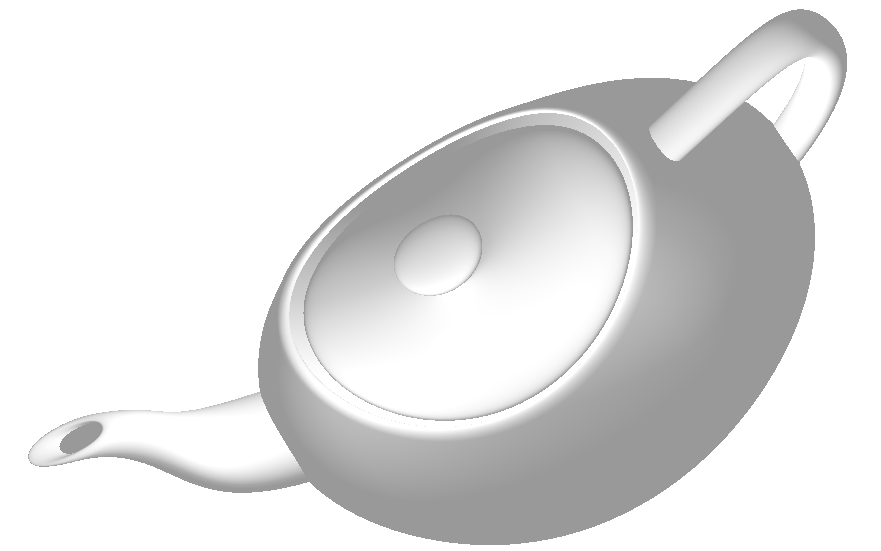
\includegraphics[width = \textwidth]{teapot1.png}
		\caption{传统自由变形结果}\label{subfig:teapot1}
	\end{subfigure}
	\begin{subfigure}[b]{.3\textwidth}
		\centering
		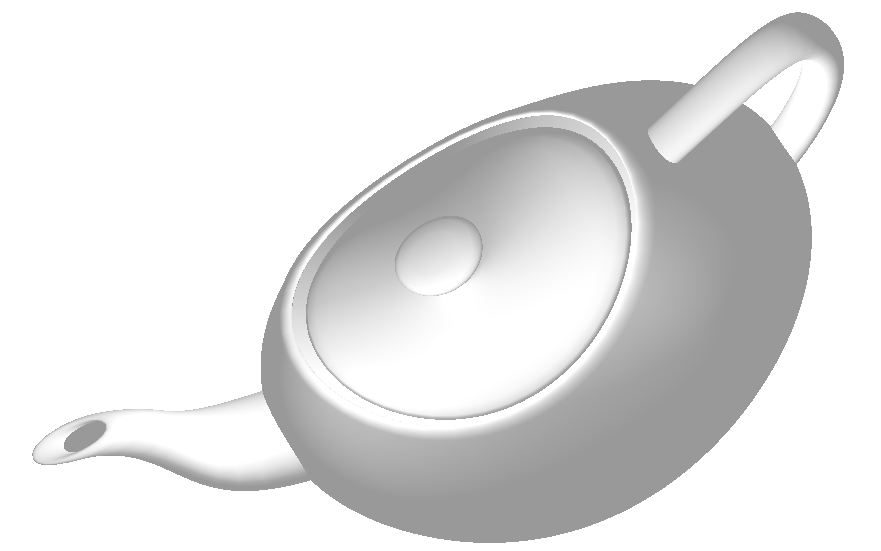
\includegraphics[width = \textwidth]{teapot2.png}
		\caption{光滑自由变形结果}\label{subfig:teapot2}
	\end{subfigure}
	\begin{subfigure}[b]{.3\textwidth}
		\centering
		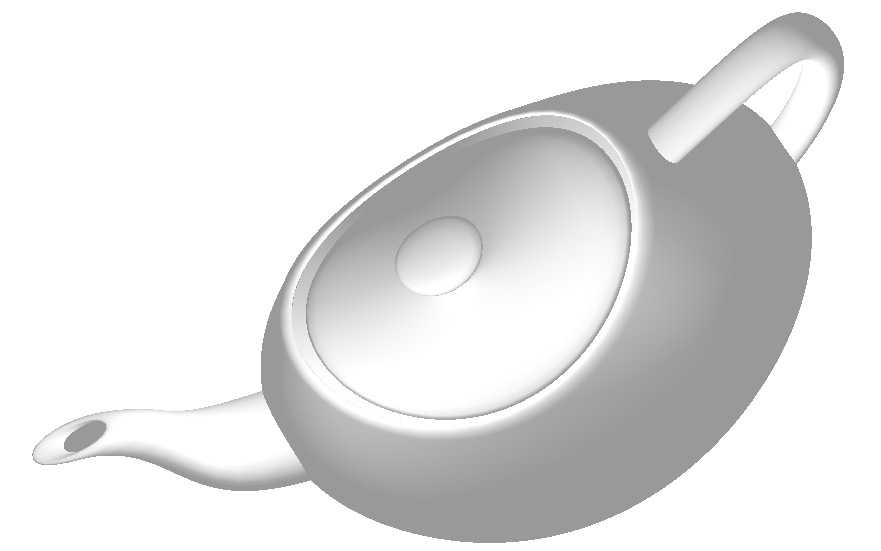
\includegraphics[width = \textwidth]{teapot3.png}
		\caption{本文结果}\label{subfig:teapot3}
	\end{subfigure}
	\caption{Utah茶壶变形结果}\label{fig:teapot_result}
\end{figure}

\autoref{subfig:cube1}是立方体模型通过精确自由变形得到的结果,该结果是精确的,所以光滑自由变形和本文方法得到的结果(如图\autoref{subfig:cube2}与\autoref{subfig:cube3}所示)都与精确自由变形得到的结果进行比较,以得到两者的变形误差,结果如\autoref{tab:error_cube}所示。其中,几何误差定义为对应点的欧氏距离,法向误差定义为对应点法向所成夹角的角度。从\autoref{tab:error_cube}中可以看出,本文方法的几何误差与法向误差均小于光滑自由变形,主要原因是本文方法选取的$l$比较小,产生的子三角形要比光滑自由变形小很多。\autoref{fig:cube_error0}、\autoref{fig:cube_error1}中是上述误差的可视化结果。

\begin{table}[htbp]
    \centering
    \caption{立方体误差} \label{tab:error_cube}
    \begin{tabular}{lrrrr}
    \toprule
                    & 平均几何误差 & 最大几何误差 & 平均法向误差 & 最大法向误差 \\
    \midrule
        本文方法    & \num{0.002952310} & \num{0.02908119} & \num[scientific-notation=false]{0.5785680}$^\circ$ & \num[scientific-notation=false]{15.89719}$^\circ$ \\
        光滑自由变形& \num{0.004904391} & \num{0.03718415} & \num[scientific-notation=false]{0.5853341}$^\circ$ & \num[scientific-notation=false]{21.24638}$^\circ$ \\
    \bottomrule
    \end{tabular}
\end{table}

\begin{figure}[htbp]
	\centering
	\begin{subfigure}[b]{.45\textwidth}
		\centering
		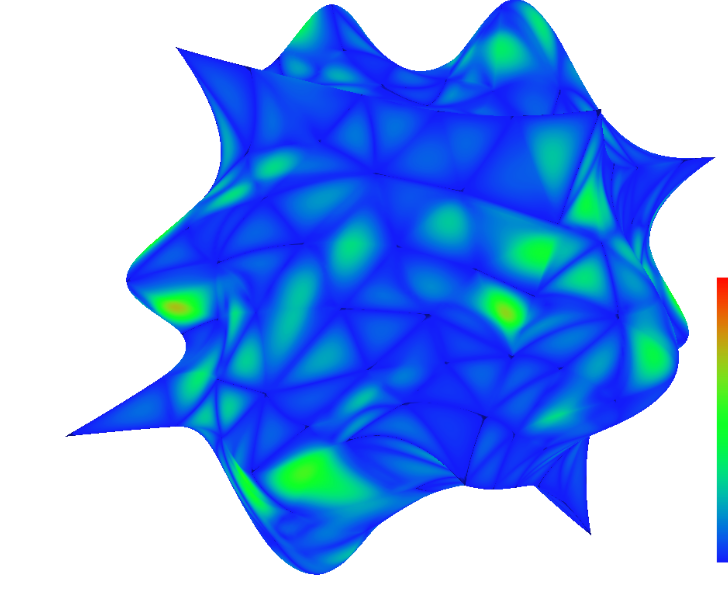
\includegraphics[width = \textwidth]{cube4.png}
		\caption{本文方法几何误差图}\label{subfig:cube4}
	\end{subfigure}%
	\begin{subfigure}[b]{.45\textwidth}
		\centering
		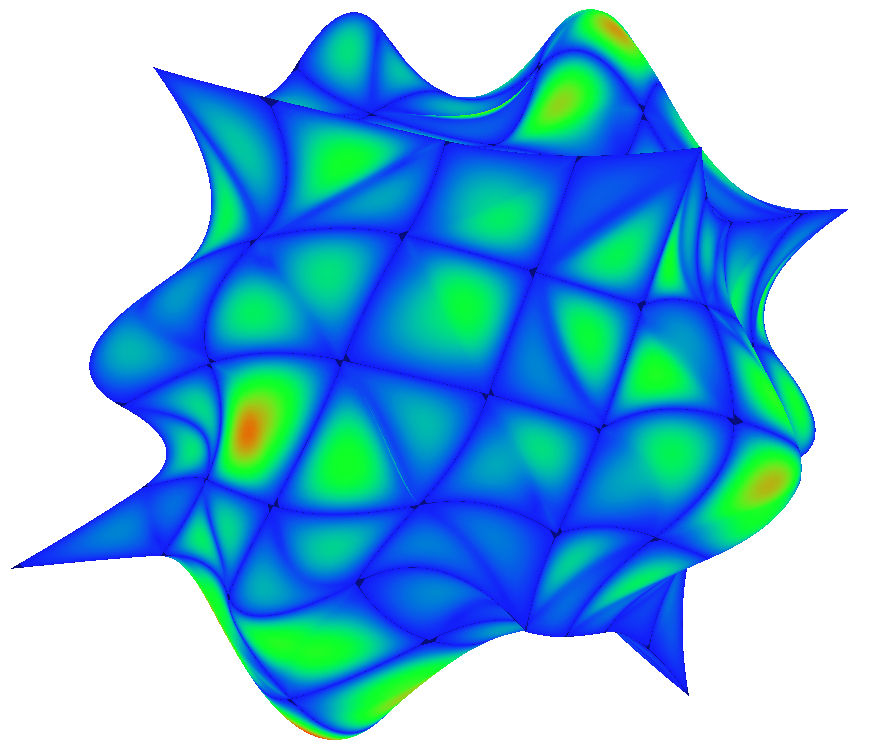
\includegraphics[width = \textwidth]{cube6.png}
		\caption{光滑自由变形几何误差图}\label{subfig:cube6}
	\end{subfigure}
	\caption{立方体几何误差}\label{fig:cube_error0}
\end{figure}
\begin{figure}[htbp]
	\centering
	\begin{subfigure}[b]{.45\textwidth}
		\centering
		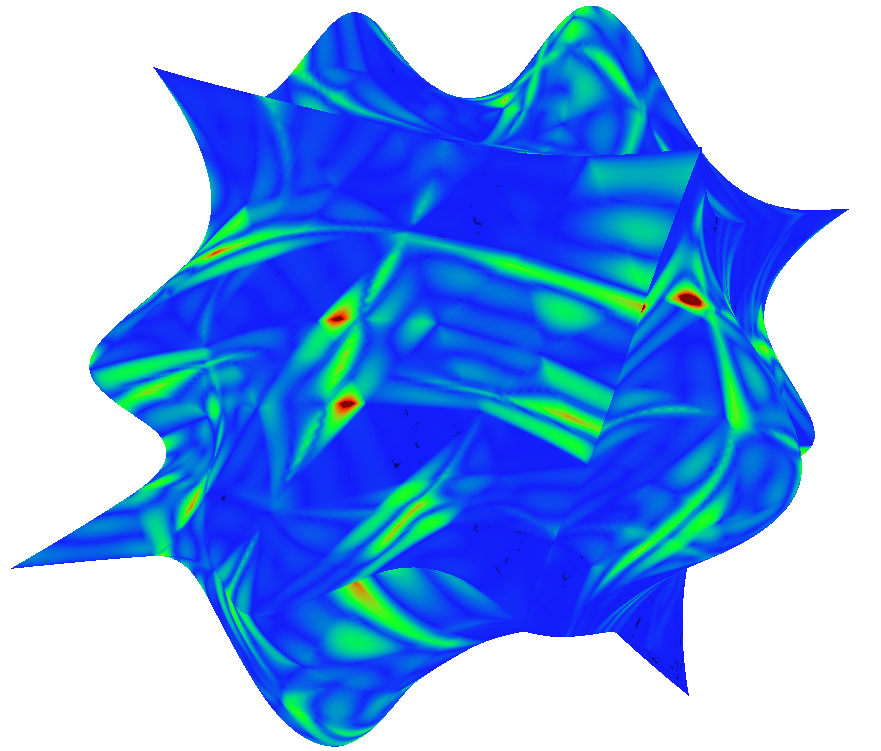
\includegraphics[width = \textwidth]{cube5.png}
		\caption{本文方法法向误差图}\label{subfig:cube5}
	\end{subfigure}%
	\begin{subfigure}[b]{.45\textwidth}
		\centering
		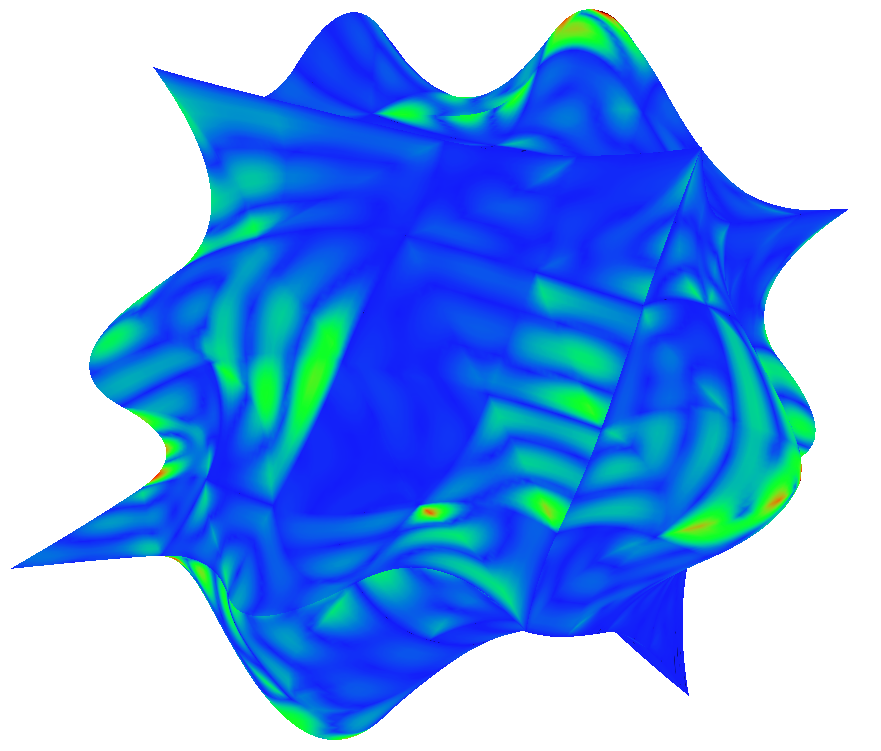
\includegraphics[width = \textwidth]{cube7.png}
		\caption{光滑自由变形法向误差图}\label{subfig:cube7}
	\end{subfigure}
	\caption{立方体法向误差}\label{fig:cube_error1}
\end{figure}

对于Utah茶壶,对比结果如\autoref{tab:error_utah}所示。我们同样给出了上述误差的可视化结果,如\autoref{fig:teapot_error0}、\autoref{fig:teapot_error1}所示。Utah茶壶经过Casteljau细分算法得到的三角形本身比较小,因此本文方法中较小的$l$没有优势,所以两种结果的几何误差和法向误差较为接近。同时从\autoref{subfig:teapot5}和\autoref{subfig:teapot7}可以看出,无论上本文方法还是光滑自由变形,曲率较大的地方法向误差都会比较大。

\begin{table}[htbp]
    \centering
    \caption{Utah茶壶误差} \label{tab:error_utah}
    \begin{tabular}{lrrrr}
    \toprule
        & 平均几何误差 & 最大几何误差 & 平均法向误差 & 最大法向误差 \\
    \midrule
        本文方法    & \num{0.006597950} & \num{0.01203453} & \num[scientific-notation=false]{0.6152188}$^\circ$ & \num[scientific-notation=false]{22.53011}$^\circ$ \\
        光滑自由变形& \num{0.006650957} & \num{0.01220984} & \num[scientific-notation=false]{0.5491496}$^\circ$ & \num[scientific-notation=false]{22.53010}$^\circ$ \\
    \bottomrule
    \end{tabular}
\end{table}

\begin{figure}[htbp]
	\centering
	\begin{subfigure}[b]{.45\textwidth}
		\centering
		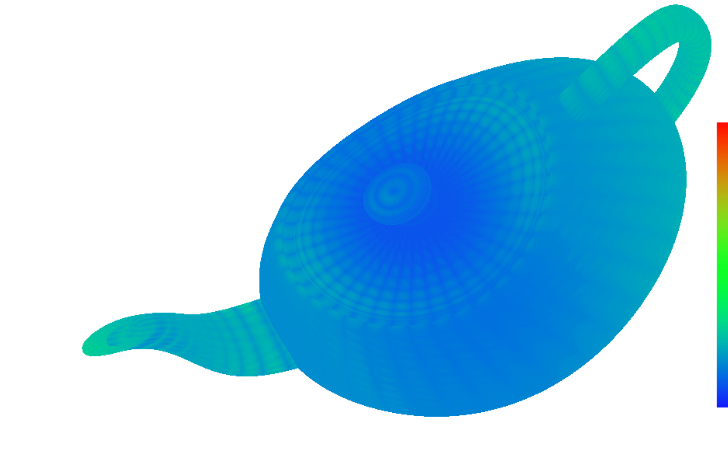
\includegraphics[width = \textwidth]{teapot4.png}
		\caption{本文方法几何误差图}\label{subfig:teapot4}
	\end{subfigure}%
	\begin{subfigure}[b]{.45\textwidth}
		\centering
		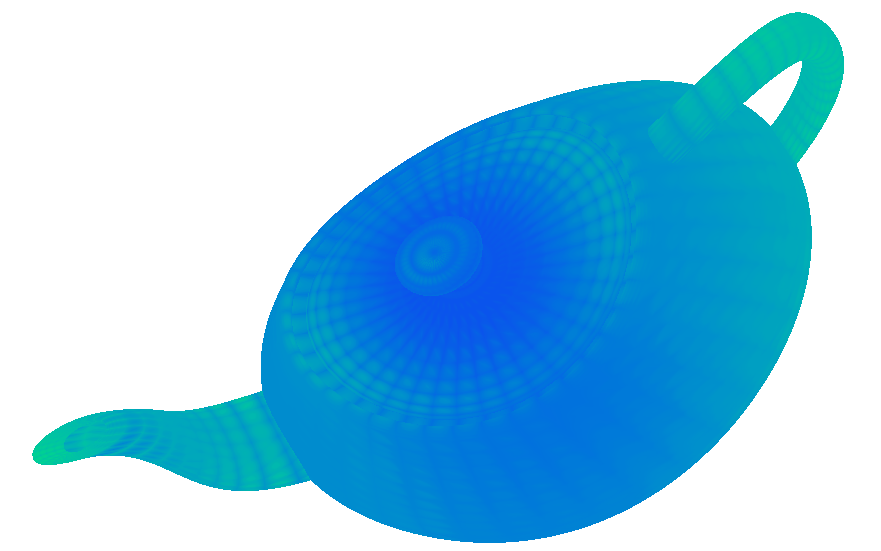
\includegraphics[width = \textwidth]{teapot6.png}
		\caption{光滑自由变形几何误差图}\label{subfig:teapot6}
	\end{subfigure}
	\caption{Utah茶壶几何误差}\label{fig:teapot_error0}
\end{figure}
\begin{figure}[htbp]
	\centering
	\begin{subfigure}[b]{.45\textwidth}
		\centering
		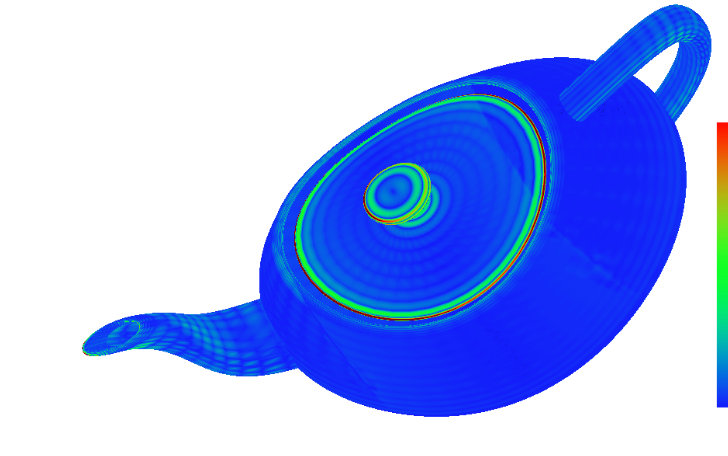
\includegraphics[width = \textwidth]{teapot5.png}
		\caption{本文方法法向误差图}\label{subfig:teapot5}
	\end{subfigure}%
	\begin{subfigure}[b]{.45\textwidth}
		\centering
		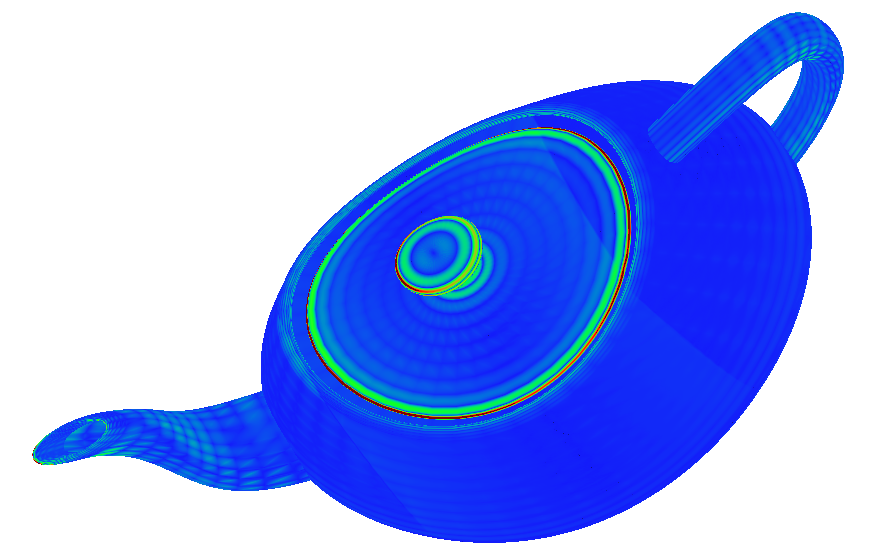
\includegraphics[width = \textwidth]{teapot7.png}
		\caption{光滑自由变形法向误差图}\label{subfig:teapot7}
	\end{subfigure}
	\caption{Utah茶壶法向误差}\label{fig:teapot_error1}
\end{figure}

\section{本章小结}
本章从绘制效果、时间效率、变形误差这三个方面对比了本文算法与同类算法。从对比结果中我们可以发现,本文算法达到了和光滑自由变形相同的变形效果,并在速度上相对于光滑自由变形算法具有一定的优势。本文算法各方面的性能均达到了我们的预期。
